\subsubsection{Module 1: Quản lý Người dùng và Xác thực}
Module này bao gồm các chức năng cốt lõi liên quan đến việc tạo lập, xác thực và quản lý tài khoản người dùng trong hệ thống.

\begin{figure}[H]
\centering
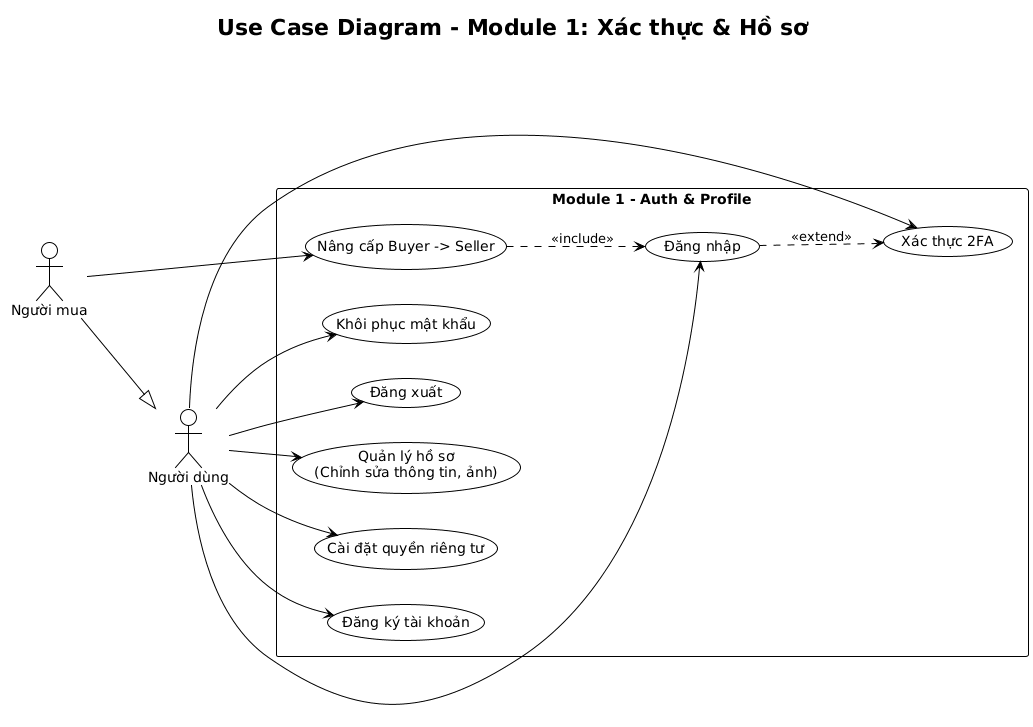
\includegraphics[width=\textwidth]{Images/Usecases/UC-M1-Auth.png}
\caption{Sơ đồ Use Case cho Module 1: Quản lý Người dùng và Xác thực}
\label{fig:usecase-module1}
\end{figure}

% Cấu hình giãn dòng cho bảng dễ đọc hơn
\renewcommand{\arraystretch}{1.3}

% =====================================================
% UC1.1: ĐĂNG KÝ TÀI KHOẢN
% =====================================================
\begin{table}[H]
\centering
\begin{tabularx}{\textwidth}{|l|X|}
\hline
\textbf{Tên Use Case} & \textbf{UC1.1: Đăng ký tài khoản} \\ \hline
\textbf{Tác nhân} & Người dùng chưa đăng nhập \\ \hline
\textbf{Mô tả} & Cho phép người dùng mới tạo một tài khoản trên hệ thống Social Commerce với vai trò mặc định là ``Người mua'' (Buyer). \\ \hline
\textbf{Kích hoạt} & Người dùng nhấn vào nút ``Đăng ký'' trên giao diện. \\ \hline
\textbf{Điều kiện tiên quyết} & 
\begin{itemize}
    \item Người dùng chưa đăng nhập vào hệ thống.
    \item Người dùng có một địa chỉ email hợp lệ và chưa được sử dụng để đăng ký.
\end{itemize} \\ \hline
\textbf{Điều kiện sau} & 
\begin{itemize}
    \item Tài khoản mới được tạo với trạng thái ``chưa xác thực''.
    \item Vai trò người dùng được gán là Buyer.
    \item Hệ thống gửi email/tin nhắn xác thực tài khoản.
    \item Người dùng được chuyển hướng đến trang yêu cầu xác thực.
\end{itemize} \\ \hline
\textbf{Luồng sự kiện chính} & 
\begin{enumerate}
    \item Người dùng truy cập trang Đăng ký.
    \item Người dùng nhập các thông tin bắt buộc.
    \item Người dùng nhấn nút ``Đăng ký''.
    \item Hệ thống kiểm tra tính hợp lệ của dữ liệu.
    \item Hệ thống kiểm tra email đã tồn tại hay chưa.
    \item Hệ thống tạo người dùng mới với trạng thái ``chưa xác thực''.
    \item Hệ thống gửi email/SMS xác thực.
    \item Hệ thống hiển thị thông báo thành công và yêu cầu xác thực.
\end{enumerate} \\ \hline
\textbf{Ngoại lệ} & 
\begin{itemize}
    \item E1: Email không hợp lệ $\rightarrow$ Báo lỗi ``Định dạng email không hợp lệ''.
    \item E2: Mật khẩu xác nhận không khớp $\rightarrow$ Báo lỗi ``Mật khẩu xác nhận không khớp''.
    \item E3: Email đã tồn tại $\rightarrow$ Báo lỗi ``Email này đã được sử dụng''.
    \item E4: Lỗi gửi email $\rightarrow$ Báo lỗi và đề nghị thử lại.
\end{itemize} \\ \hline
\textbf{Ghi chú} & Đây là bước đầu tiên để tham gia vào hệ sinh thái Social Commerce. \\ \hline
\end{tabularx}
\caption{Đặc tả Use Case Đăng ký tài khoản}
\end{table}

% =====================================================
% UC1.2: ĐĂNG NHẬP
% =====================================================
\begin{table}[H]
\centering
\begin{tabularx}{\textwidth}{|l|X|}
\hline
\textbf{Tên Use Case} & \textbf{UC1.2: Đăng nhập vào hệ thống} \\ \hline
\textbf{Tác nhân} & Người dùng chưa đăng nhập \\ \hline
\textbf{Mô tả} & Cho phép người dùng đã có tài khoản truy cập vào hệ thống bằng email và mật khẩu. \\ \hline
\textbf{Kích hoạt} & Người dùng nhấn vào nút ``Đăng nhập'' sau khi điền thông tin. \\ \hline
\textbf{Điều kiện tiên quyết} & Người dùng có một tài khoản đã đăng ký và xác thực. \\ \hline
\textbf{Điều kiện sau} & 
\begin{itemize}
    \item Hệ thống tạo một phiên làm việc (session) cho người dùng.
    \item Hệ thống cấp một JSON Web Token (JWT) để xác thực.
    \item Người dùng được chuyển hướng đến trang chủ.
\end{itemize} \\ \hline
\textbf{Luồng sự kiện chính} & 
\begin{enumerate}
    \item Người dùng truy cập trang Đăng nhập.
    \item Người dùng nhập email và mật khẩu.
    \item Người dùng nhấn nút ``Đăng nhập''.
    \item Hệ thống xác thực thông tin.
    \item Nếu thông tin chính xác và tài khoản không bật 2FA, hệ thống tạo JWT và chuyển hướng người dùng.
\end{enumerate} \\ \hline
\textbf{Ngoại lệ} & 
\begin{itemize}
    \item E1: Sai email hoặc mật khẩu $\rightarrow$ Báo lỗi ``Thông tin đăng nhập không chính xác''.
    \item E2: Tài khoản chưa được xác thực $\rightarrow$ Báo lỗi và yêu cầu xác thực.
    \item E3: Tài khoản bị khóa $\rightarrow$ Báo lỗi ``Tài khoản của bạn đã bị khóa''.
\end{itemize} \\ \hline
\textbf{Ghi chú} & Quá trình xác thực sử dụng JWT để đảm bảo an toàn. \\ \hline
\end{tabularx}
\caption{Đặc tả Use Case Đăng nhập}
\end{table}

% =====================================================
% UC1.3: XÁC THỰC 2 YẾU TỐ (2FA)
% =====================================================
\begin{table}[H]
\centering
\begin{tabularx}{\textwidth}{|l|X|}
\hline
\textbf{Tên Use Case} & \textbf{UC1.3: Sử dụng xác thực hai yếu tố (2FA)} \\ \hline
\textbf{Tác nhân} & Người dùng \\ \hline
\textbf{Mô tả} & Cung cấp một lớp bảo mật bổ sung khi đăng nhập bằng mã xác thực tạm thời. \\ \hline
\textbf{Kích hoạt} & Người dùng có bật 2FA và vừa nhập đúng mật khẩu ở bước đăng nhập. \\ \hline
\textbf{Điều kiện tiên quyết} & 
\begin{itemize}
    \item Người dùng đã kích hoạt tính năng 2FA.
    \item Người dùng đã nhập chính xác email và mật khẩu.
\end{itemize} \\ \hline
\textbf{Điều kiện sau} & 
\begin{itemize}
    \item Danh tính người dùng được xác thực hoàn toàn.
    \item Người dùng được đăng nhập thành công.
\end{itemize} \\ \hline
\textbf{Luồng sự kiện chính} & 
\begin{enumerate}
    \item Hệ thống hiển thị trang nhập mã 2FA.
    \item Người dùng lấy mã từ email (hoặc ứng dụng Authenticator).
    \item Người dùng nhập mã 2FA.
    \item Người dùng nhấn ``Xác nhận''.
    \item Hệ thống kiểm tra mã.
    \item Nếu mã hợp lệ, quá trình đăng nhập hoàn tất.
\end{enumerate} \\ \hline
\textbf{Ngoại lệ} & 
\begin{itemize}
    \item E1: Nhập sai mã 2FA $\rightarrow$ Báo lỗi ``Mã xác thực không chính xác''.
    \item E2: Mã 2FA hết hạn $\rightarrow$ Báo lỗi và yêu cầu thử lại.
\end{itemize} \\ \hline
\textbf{Ghi chú} & Tính năng này tùy chọn và quan trọng cho tài khoản người bán. \\ \hline
\end{tabularx}
\caption{Đặc tả Use Case Xác thực 2FA}
\end{table}

% =====================================================
% UC1.4: KHÔI PHỤC MẬT KHẨU
% =====================================================
\begin{table}[H]
\centering
\begin{tabularx}{\textwidth}{|l|X|}
\hline
\textbf{Tên Use Case} & \textbf{UC1.4: Khôi phục mật khẩu} \\ \hline
\textbf{Tác nhân} & Người dùng chưa đăng nhập \\ \hline
\textbf{Mô tả} & Cho phép người dùng đặt lại mật khẩu trong trường hợp họ quên. \\ \hline
\textbf{Kích hoạt} & Người dùng nhấn vào liên kết ``Quên mật khẩu?'' trên trang Đăng nhập. \\ \hline
\textbf{Điều kiện tiên quyết} & 
\begin{itemize}
    \item Người dùng có một tài khoản đã đăng ký.
    \item Người dùng có quyền truy cập vào email đã đăng ký.
\end{itemize} \\ \hline
\textbf{Điều kiện sau} & Mật khẩu của người dùng được cập nhật thành công. \\ \hline
\textbf{Luồng sự kiện chính} & 
\begin{enumerate}
    \item Người dùng nhấn ``Quên mật khẩu?''.
    \item Hệ thống yêu cầu người dùng nhập email.
    \item Người dùng nhập email và nhấn ``Gửi''.
    \item Hệ thống gửi email chứa liên kết hoặc mã OTP.
    \item Người dùng làm theo hướng dẫn trong email.
    \item Hệ thống chuyển hướng đến trang tạo mật khẩu mới.
    \item Người dùng nhập mật khẩu mới và xác nhận.
    \item Người dùng nhấn ``Lưu thay đổi''.
    \item Hệ thống cập nhật mật khẩu và thông báo thành công.
\end{enumerate} \\ \hline
\textbf{Ngoại lệ} & 
\begin{itemize}
    \item E1: Email không tồn tại $\rightarrow$ Hệ thống hiển thị thông báo chung để bảo mật (tránh lộ danh tính user).
    \item E2: Liên kết/mã OTP hết hạn hoặc không hợp lệ $\rightarrow$ Báo lỗi và yêu cầu làm lại.
    \item E3: Mật khẩu mới không khớp $\rightarrow$ Báo lỗi.
\end{itemize} \\ \hline
\end{tabularx}
\caption{Đặc tả Use Case Khôi phục mật khẩu}
\end{table}

% =====================================================
% UC1.5: ĐĂNG XUẤT
% =====================================================
\begin{table}[H]
\centering
\begin{tabularx}{\textwidth}{|l|X|}
\hline
\textbf{Tên Use Case} & \textbf{UC1.5: Đăng xuất} \\ \hline
\textbf{Tác nhân} & Người dùng \\ \hline
\textbf{Mô tả} & Cho phép người dùng kết thúc phiên làm việc hiện tại một cách an toàn. \\ \hline
\textbf{Kích hoạt} & Người dùng nhấn vào nút ``Đăng xuất''. \\ \hline
\textbf{Điều kiện tiên quyết} & Người dùng đang đăng nhập vào hệ thống. \\ \hline
\textbf{Điều kiện sau} & 
\begin{itemize}
    \item Phiên làm việc của người dùng bị hủy.
    \item JWT trên client bị xóa.
    \item Người dùng được chuyển hướng về trang chủ.
\end{itemize} \\ \hline
\textbf{Luồng sự kiện chính} & 
\begin{enumerate}
    \item Người dùng nhấn nút ``Đăng xuất''.
    \item Hệ thống hủy phiên làm việc và xóa token lưu trữ ở client.
    \item Hệ thống chuyển hướng người dùng về trang chủ.
\end{enumerate} \\ \hline
\end{tabularx}
\caption{Đặc tả Use Case Đăng xuất}
\end{table}

% =====================================================
% UC1.6: QUẢN LÝ HỒ SƠ CÁ NHÂN
% =====================================================
\begin{table}[H]
\centering
\begin{tabularx}{\textwidth}{|l|X|}
\hline
\textbf{Tên Use Case} & \textbf{UC1.6: Quản lý hồ sơ cá nhân} \\ \hline
\textbf{Tác nhân} & Người dùng \\ \hline
\textbf{Mô tả} & Cho phép người dùng xem và chỉnh sửa thông tin cá nhân, ảnh đại diện và ảnh bìa. \\ \hline
\textbf{Kích hoạt} & Người dùng truy cập trang cá nhân và chọn chức năng chỉnh sửa. \\ \hline
\textbf{Điều kiện tiên quyết} & Người dùng đang đăng nhập vào hệ thống. \\ \hline
\textbf{Điều kiện sau} & 
\begin{itemize}
    \item Thông tin cá nhân của người dùng được cập nhật.
    \item Thay đổi được hiển thị ngay lập tức.
\end{itemize} \\ \hline
\textbf{Luồng sự kiện chính} & 
\begin{enumerate}
    \item Người dùng vào trang hồ sơ cá nhân.
    \item Người dùng nhấn ``Chỉnh sửa hồ sơ''.
    \item Người dùng thay đổi thông tin.
    \item Người dùng nhấn ``Lưu thay đổi''.
    \item Hệ thống xác thực và cập nhật dữ liệu.
    \item Hệ thống hiển thị thông báo thành công.
\end{enumerate} \\ \hline
\textbf{Luồng thay thế} & A1: Người dùng nhấn ``Hủy'' $\rightarrow$ Các thay đổi sẽ không được lưu. \\ \hline
\textbf{Ngoại lệ} & 
\begin{itemize}
    \item E1: Lỗi tải lên hình ảnh $\rightarrow$ Báo lỗi tương ứng.
    \item E2: Dữ liệu nhập không hợp lệ $\rightarrow$ Báo lỗi tại trường dữ liệu đó.
\end{itemize} \\ \hline
\textbf{Ghi chú} & Giao diện quản lý cần trực quan và dễ sử dụng. \\ \hline
\end{tabularx}
\caption{Đặc tả Use Case Quản lý hồ sơ}
\end{table}

% =====================================================
% UC1.7: CÀI ĐẶT QUYỀN RIÊNG TƯ
% =====================================================
\begin{table}[H]
\centering
\begin{tabularx}{\textwidth}{|l|X|}
\hline
\textbf{Tên Use Case} & \textbf{UC1.7: Cài đặt quyền riêng tư cho tài khoản} \\ \hline
\textbf{Tác nhân} & Người dùng \\ \hline
\textbf{Mô tả} & Cho phép người dùng tùy chỉnh ai có thể xem hồ sơ, bài đăng hoặc danh sách người theo dõi. \\ \hline
\textbf{Kích hoạt} & Người dùng truy cập vào mục ``Cài đặt \& Quyền riêng tư''. \\ \hline
\textbf{Điều kiện tiên quyết} & Người dùng đang đăng nhập vào hệ thống. \\ \hline
\textbf{Điều kiện sau} & Các thiết lập quyền riêng tư của người dùng được cập nhật. \\ \hline
\textbf{Luồng sự kiện chính} & 
\begin{enumerate}
    \item Người dùng vào trang ``Cài đặt''.
    \item Người dùng chọn tab ``Quyền riêng tư''100.
    \item Người dùng thay đổi các tùy chọn.
    \item Người dùng nhấn ``Lưu thay đổi''.
    \item Hệ thống cập nhật và hiển thị thông báo thành công.
\end{enumerate} \\ \hline
\textbf{Ghi chú} & Tính năng này quan trọng để người dùng cảm thấy an toàn và kiểm soát thông tin. \\ \hline
\end{tabularx}
\caption{Đặc tả Use Case Cài đặt quyền riêng tư}
\end{table}

% =====================================================
% UC1.8: ĐĂNG KÝ NGƯỜI BÁN
% =====================================================
\begin{table}[H]
\centering
\begin{tabularx}{\textwidth}{|l|X|}
\hline
\textbf{Tên Use Case} & \textbf{UC1.8: Đăng ký trở thành Người bán} \\ \hline
\textbf{Tác nhân} & Người dùng (với vai trò Buyer) \\ \hline
\textbf{Mô tả} & Cung cấp quy trình để người dùng ``Người mua'' nâng cấp tài khoản thành ``Người bán''. \\ \hline
\textbf{Kích hoạt} & Người dùng nhấn vào nút ``Trở thành người bán''. \\ \hline
\textbf{Điều kiện tiên quyết} & 
\begin{itemize}
    \item Người dùng đang đăng nhập.
    \item Người dùng hiện có vai trò là Buyer.
\end{itemize} \\ \hline
\textbf{Điều kiện sau} & 
\begin{itemize}
    \item Hồ sơ đăng ký Seller được lưu và chuyển sang trạng thái chờ duyệt (\textit{REVIEWING}) sau khi hoàn thành các bước bắt buộc.
    \item Khi Admin phê duyệt, vai trò người dùng được cập nhật thành Seller.
\end{itemize} \\ \hline
\textbf{Luồng sự kiện chính} & 
\begin{enumerate}
    \item Người dùng truy cập trang ``Đăng ký Bán hàng'' và bắt đầu hồ sơ.
    \item Người dùng hoàn thành bước 1 (thông tin cá nhân/định danh).
    \item Người dùng hoàn thành bước 2 (thông tin kinh doanh).
    \item Người dùng hoàn thành bước 3 (thông tin ngân hàng) và nộp hồ sơ.
    \item Hệ thống chuyển hồ sơ sang trạng thái ``Đang xem xét''.
    \item Admin xét duyệt hồ sơ.
    \item Nếu được duyệt, hệ thống cập nhật vai trò thành Seller và gửi thông báo kết quả.
\end{enumerate} \\ \hline
\textbf{Luồng thay thế} & A1: Người dùng hủy bỏ quá trình đăng ký. \\ \hline
\textbf{Ngoại lệ} & 
\begin{itemize}
    \item E1: Thông tin ở bất kỳ bước nào không hợp lệ $\rightarrow$ Báo lỗi và yêu cầu sửa.
    \item E2: Hồ sơ bị từ chối $\rightarrow$ Hiển thị lý do từ chối để người dùng bổ sung.
\end{itemize} \\ \hline
\textbf{Ghi chú} & Đây là use case cốt lõi thể hiện mô hình ``buyer-to-seller'' của dự án. \\ \hline
\end{tabularx}
\caption{Đặc tả Use Case Đăng ký làm Người bán}
\end{table}